\chapter{Codifica con distorsione}

Consideriamo ora il problema di ricostruire il canale di DL
\(\bm{h}^\mathrm{(D)}\) alla BS in presenza di una data distorsione \(d\).
Anche in questo caso ci concentriamo inizialmente sul caso senza feedforward
(\(b_\mathrm{F} = 0\)).

\begin{figure}[ht]
    \centering
    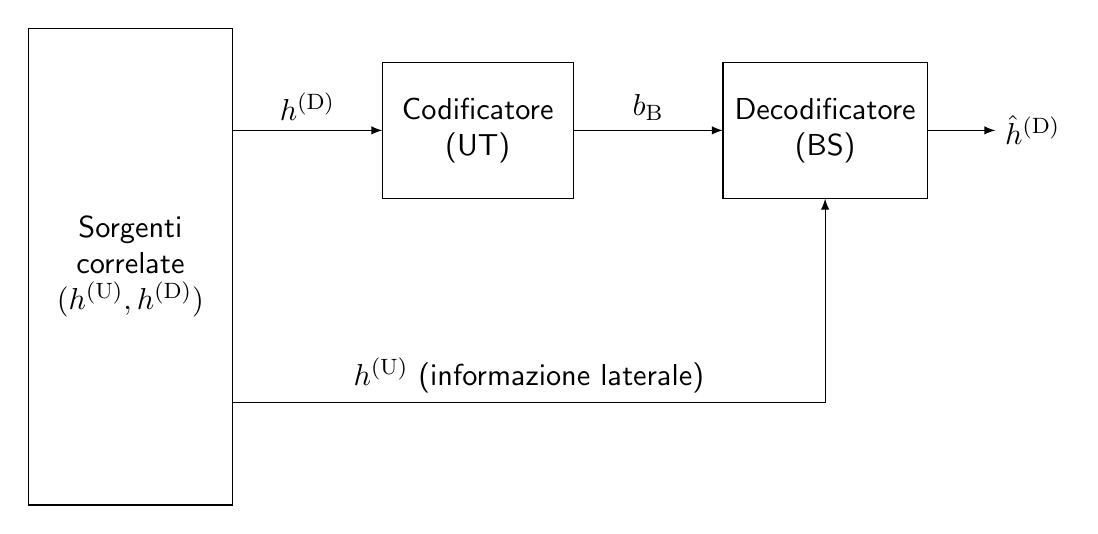
\begin{tikzpicture}[scale=0.865,>=latex]
    \tikzstyle{every node}=[font=\fontsize{11}{13}\sffamily]

    \draw (0,0) rectangle (3,7)
    node[midway,align=center]
    {Sorgenti \\ correlate \\ \((\bm{h}^\mathrm{(U)},\bm{h}^\mathrm{(D)})\)};

    \draw[->] (3,5.5) -- (5.2,5.5)
    node[above,midway]{\(\bm{h}^\mathrm{(D)}\)};

    \draw[-] (3,1.5) -- (11.7,1.5)
    node[above,midway]{\(\bm{h}^\mathrm{(U)}\) (informazione laterale)};

    \draw[->] (11.7,1.5) -- (11.7,4.5);

    \draw (5.2,4.5) rectangle (8,6.5)
    node[midway,align=center]{Codificatore \\ (UT)};

    \draw[->] (8,5.5) -- (10.2,5.5)
    node[above,midway]{\(b_\mathrm{B}\)};

    \draw (10.2,4.5) rectangle (13.2,6.5)
    node[midway,align=center]{Decodificatore \\ (BS)};

    \draw[->] (13.2,5.5) -- (14.2,5.5)
    node[right]{\(\hat{\bm{h}}^\mathrm{(D)}\)};
\end{tikzpicture}

    \caption{
        Configurazione del sistema per la codifica di sorgente in presenza di
        informazione laterale.
    }
    \label{fig:wz-configuration}
\end{figure}

Anzitutto, poiché una stima del canale di UL è già presente alla base station,
possiamo vedere lo scenario considerato come una codifica di sorgenti correlate
distribuite (i canali di UL e DL) in presenza di informazione laterale (il canale di
uplink \(\bm{h}^\mathrm{(U)}\) già noto alla BS). Desideriamo quindi utilizzare
l'informazione laterale, nota solo al decodificatore (la BS nel nostro caso),
per ridurre il tasso di trasmissione \(b_\mathrm{B}\) necessario per effettuare
una trasmissione del canale di downlink \(\bm{h}^\mathrm{(D)}\) che risulti
affidabile anche in presenza della suddetta distorsione \(d\). La situazione
appena descritta è rappresentata in Figura~\ref{fig:wz-configuration}.

Un'estensione del teorema di Slepian-Wolf (Teorema~\ref{thm:sw}) che consideri
la presenza di distorsione è possibile grazie al lavoro di Wyner e Ziv. Di
seguito, riportiamo la descrizione formale del problema considerato, e
successivamente il teorema di Wyner-Ziv.\cite{1055508}

Detto \(\set{U}\) un insieme finito arbitrario, sia \(\set{U}^n\) l'insieme dei
vettori di \(n\) elementi con valori in \(\set{U}\). Denotiamo con \(\bm{X}^n\)
un vettore aleatorio di cardinalità \(n\). Per \(k=1,2,\dots\), definiamo
l'insieme
\begin{equation}
    I_k = \{0,1,2,\dots,k-1\}.
\end{equation}
Siano \(\set{X},\set{Y},\hat{\set{X}}\) insiemi finiti e sia
\(\{(X_k,Y_k)\}_1^\infty\) una sequenza di estrazioni indipendenti di una
coppia di variabili aleatorie dipendenti \(X,Y\) con valori in \(\set{X}\) e
\(\set{Y}\), rispettivamente. La distribuzione di probabilità per la coppia
\(X,Y\) è data da
\begin{equation}
    Q(x,y) = \prob{X = x, Y = y}, \quad x \in \set{X}, y \in \set{Y}.
\end{equation}

Sia \(D: \set{X}\times\hat{\set{X}} \to [0,\infty)\) una funzione di
distorsione. Un codice \((n,M,\Delta)\) è definito da una coppia di funzioni
\(F_\mathrm{E},F_\mathrm{D}\), un "codificatore" e un "decodificatore",
rispettivamente, dove
\begin{alignat}{1}
    F_\mathrm{E}: \set{X}^n \to I_M &, \\
    F_\mathrm{D}: \set{Y}^n \times I_M \to \hat{\set{X}}^n &,
\end{alignat}
e
\begin{equation}
    \expect{\frac{1}{n} \sum_{k=1}^n D(X_k,\hat{X}_k)} = \Delta,
\end{equation}
dove \(\hat{\bm{X}}^n = F_\mathrm{D}(\bm{Y}^n,F_\mathrm{E}(\bm{X}^n))\).
Diciamo che una coppia \((R,d)\) è ottenibile se, per \(\varepsilon > 0\) a
piacere, esiste (per \(n\) sufficientemente grande) un codice \((n,M,\Delta)\)
con
\begin{equation}
    M \le 2^{n (R + \varepsilon)}, \quad \Delta \le d + \varepsilon .
\end{equation}
Definiamo con \(\set{R}\) l'insieme delle coppie \((R,d)\) ottenibili, e
definiamo
\begin{equation}
    R^{*}(d) = \min_{(R,d)\,\in\,\set{R}} R . \label{eq:r-star}
\end{equation}
Poiché, per la definizione data, \(\set{R}\) è un insieme chiuso, il minimo
indicato nella definizione di \(R^{*}(d)\) esiste. Inoltre, dal momento che
\(R^{*}(d)\) è una funzione non crescente in \(d\), abbiamo \(R^{*}(0) \ge
\lim_{d\to0} R^{*}(d)\). Per di più, dalla \eqref{eq:r-star}, per tutti i
valori di \(d \ge 0\), la coppia \((R^{*}(d), d) \in \set{R}\). Infine, dal
momento che \(\set{R}\) è chiuso, \((\lim_{d\to0} R^{*}(d), 0) \in \set{R}\), e
abbiamo che \(R^{*}(0) \le \lim_{d\to0} R^{*}(d)\). Concludiamo quindi che
\(R^{*}(d)\) è continua in \(d = 0\).

Sia \(p(x,y,z), x \in \set{X}, y \in \set{Y}, z \in \set{Z}\), dove \(\set{Z}\)
è un insieme finito arbitrario, una distribuzione di probabilità che definisce
le variabili aleatorie \(X,Y,Z\), tali che la distribuzione marginale per
\(X,Y\) è
\begin{equation}
    \sum_{z \in \set{Z}} p(x,y,z) = Q(x,y) \label{eq:wz-distr-constr-1}
\end{equation}
e tale che
\begin{equation}
    Y,Z \textrm{ sono condizionate indipendentemente data } X.
    \label{eq:wz-distr-constr-2}
\end{equation}
Ora, per \(d > 0\), definiamo \(\set{M}(d)\) come l'insieme delle distribuzioni
di probabilità \(p(x,y,z)\) che soddisfa \eqref{eq:wz-distr-constr-1} e
\eqref{eq:wz-distr-constr-2}, e che ha la proprietà che esiste una funzione
\(f: \set{Y}\times\set{X} \to \hat{\set{X}}\) tale che
\begin{equation}
    \expect{D(X,\hat{X})} \le d, \quad
    \textrm{dove } \hat{X} = f(Y,Z) .
\end{equation}

\begin{thm}[Wyner-Ziv \textnormal{\cite{1055508}}]
    \label{thm:wz}

    Definiamo, per \(d > 0\), la quantità
    \begin{equation}
        \bar{R}(d) \define \inf_{p\,\in\,\set{M}(d)} \mleft[
            \mutual{X}{Z} - \mutual{Y}{Z}
            \mright]
        = \inf_{p\,\in\,\set{M}(d)} \mutual{X}{Z \given Y} .
    \end{equation}
    Poiché \(\set{M}(d_1) \subseteq \set{M}(d_2)\) per tutti i valori di \(d_1
    < d_2\), \(\bar{R}(d)\) è non crescente, per \(d \in (0,\infty)\). Quindi,
    possiamo definire
    \begin{equation}
        \bar{R}(0) = \lim_{d\to0} \bar{R}(d) .
    \end{equation}
    Per \(d \ge 0\), si ha
    \begin{equation}
        R^{*}(d) = \bar{R}(d) .
    \end{equation}
\end{thm}

Il teorema di Wyner-Ziv ci dice quindi che, in presenza di distorsione \(d\),
possiamo effettuare la trasmissione del canale di DL dallo UT alla BS con un
tasso
\begin{equation}
    b_\mathrm{B} \ge \inf_{p\,\in\,\set{M}(d)}
    \mutual{\bm{h}^\mathrm{(D)}}{Z \given \bm{h}^\mathrm{(U)}} ,
    \label{eq:rate-with-wz}
\end{equation}
dove la variabile aleatoria ausiliaria \(Z \in \set{Z}\), con \(\set{Z}\)
insieme finito, deve soddisfare i vincoli: i) \(\bm{h}^\mathrm{(U)},Z\) sono
indipendenti dato \(\bm{h}^\mathrm{(D)}\); ii) esiste una funzione \(f: \set{V}
\times \set{Z} \to \hat{\set{D}}\), tale che \(\expect{D(\bm{h}^\mathrm{(D)},
f(\bm{h}^\mathrm{(U)},Z))} \le d\), dove \(\hat{\set{D}}\) è l'alfabeto in cui
prende valori la versione ricevuta alla BS del canale di DL.

Nella pratica, risultati simili al limite teorico \eqref{eq:rate-with-wz} si
possono ottenere, ad esempio, utilizzando una codifica tramite sindrome che
sfrutti la presenza dell'informazione laterale, ovvero la stima di
\(\bm{h}^\mathrm{(U)}\) nota al decodificatore, la BS. A questo proposito, si
veda il lavoro di S.S. Pradhan e K. Ramachandran\cite{1184140}.

\section{Codifica con feedforward}
\label{sec:with-feedforward}

Nel caso in cui si permette una distorsione nella ricostruzione del canale alla
BS, la trasmissione di un segnale di feedforward può ridurre il tasso di
feedback. Si noti che questo non avveniva nel caso senza distorsione, come
dimostrato nella Sezione~\ref{sec:feedback-only}.

Supponiamo in particolare che la BS trasmetta allo UT una descrizione di
\(\bm{h}^\mathrm{(U)}\) senza distorsione, quindi che in fase di codifica lo UT
conosca perfettamente sia \(\bm{h}^\mathrm{(D)}\) che \(\bm{h}^\mathrm{(U)}\).
In questo caso abbiamo un problema di teoria della distorsione condizionata
(\textit{Conditional Rate-Distortion Theory}). Usando le definizioni introdotte
nella sezione precedente, in questo caso si ha \cite{Gray1972ConditionalRT} che
\begin{equation}
    b_\mathrm{B} \ge \inf_{p(
        \hat{\bm{h}}^\mathrm{(D)} \mid \bm{h}^\mathrm{(D)}, \bm{h}^\mathrm{(U)}
    )}
    \mutual{
        \bm{h}^\mathrm{(D)}
    }{
        \hat{\bm{h}}^\mathrm{(D)} \given \bm{h}^\mathrm{(U)}
    } , \label{eq:rate-with-wz-and-feedforward}
\end{equation}
dove \(\hat{\bm{h}}^\mathrm{(D)}\) è la versione distorta di
\(\bm{h}^\mathrm{(D)}\) ottenuta al decodificatore, ovvero alla base station.

Usando ipotesi più stringenti, supponiamo ora che la BS trasmetta allo UT una
descrizione del canale di UL quantizzata \(q(\bm{h}^\mathrm{(U)})\). Questa
condizione corrisponde al caso reale, infatti la quantizzazione è necessaria
essendo \(\bm{q}^\mathrm{(U)}\) a valori continui. In questo caso la
rappresentazione del canale di UL allo UT è imperfetta, e abbiamo allora un
problema di distorsione con informazione laterale mista
(\textit{Rate-Distortion With Mixed Types of Side Information}) e si ha
\cite{1614094} che
\begin{equation}
    b_\mathrm{B} \ge \inf_{W \in \set{M}_{
        \bm{h}^\mathrm{(D)} \mid \bm{h}^\mathrm{(U)} \{Z\}
    }(p, D)} \mutual{
        \bm{h}^\mathrm{(D)}
    }{
        W \given \bm{h}^\mathrm{(U)} \:,\; Z
    } , \label{eq:rate-with-wz-mixed-si}
\end{equation}
dove \(\set{M}_{\bm{h}^\mathrm{(D)} \mid \bm{h}^\mathrm{(U)} \{Z\}}(p, D)\) è
l'insieme di tutte le variabili aleatorie \(W\) descritte da un canale di test
con la proprietà che \(W \to (\bm{h}^\mathrm{(D)}, \bm{h}^\mathrm{(U)}) \to Z\)
e per le quali esiste una funzione \(f: \set{W} \times \set{U} \times \set{Z}
\to \hat{\set{D}}\) tale che
\begin{equation}
    \expect{D(\bm{h}^\mathrm{(D)}, \hat{\bm{h}^\mathrm{(D)}})} \le d, \quad
    \textrm{dove } \hat{\bm{h}^\mathrm{(D)}} = f(W, \bm{h}^\mathrm{(U)}, Z) .
\end{equation}


\section{Da Mixed Side Information a Wyner-Ziv}
\label{sec:msi-system-to-wz}

\begin{prop}
    \label{prop:msi-to-wz}

    Sia \(X\) la sorgente codificata da un sistema Mixed Side Information
    \cite{1614094}. Sia \(Y\) l'informazione laterale nota sia al codificatore
    che al decodificatore di questo sistema e \(Z\) l'informazione laterale
    nota al solo decodificatore. Tale sistema può essere ridotto a un sistema
    Wyner-Ziv \cite{1055508} dove la sorgente è \(X'=X,Y\) e l'informazione
    laterale (nota al solo decodificatore) è \(Z'=Y,Z\).
\end{prop}

\begin{figure}[hb]
    \centering
    \begin{subfigure}[b]{0.45\textwidth}
        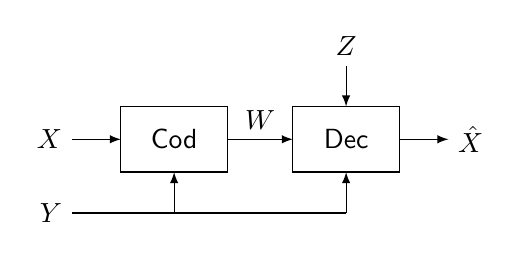
\begin{tikzpicture}[scale=0.52,>=latex]
    \tikzstyle{every node}=[font=\fontsize{10}{12}\sffamily]

    \draw[->] (0,0.8) node[left]{\(X\)} -- (1.2,0.8);

    \draw (1.2,0) rectangle (3.8,1.6)
    node[midway,align=center]{Cod};

    \draw[->] (3.8,0.8) -- (5.4,0.8)
    node[above,midway]{\(W\)};

    \draw (5.4,0) rectangle (8,1.6)
    node[midway,align=center]{Dec};

    \draw[->] (8,0.8) -- (9.2,0.8)
    node[right]{\(\hat{X}\)};

    \draw[<-] (6.7,1.6) -- (6.7,2.6)
    node[above]{\(Z\)};

    \draw[-] (0,-1) node[left]{\(Y\)} -- (6.7,-1);
    \draw[->] (2.5,-1) -- (2.5,0);
    \draw[->] (6.7,-1) -- (6.7,0);
\end{tikzpicture}

        \caption{}
        \label{fig:mini-msi}
    \end{subfigure}
    \begin{subfigure}[b]{0.54\textwidth}
        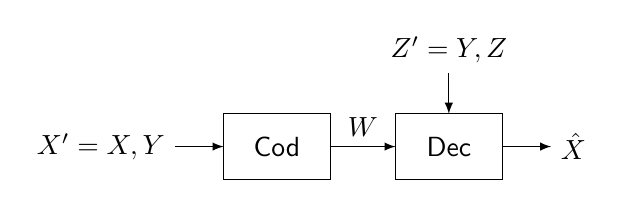
\begin{tikzpicture}[scale=0.52,>=latex]
    \tikzstyle{every node}=[font=\fontsize{10}{12}\sffamily]

    \draw[->] (0,0.8) node[left]{\(X'=X,Y\)} -- (1.2,0.8);

    \draw (1.2,0) rectangle (3.8,1.6)
    node[midway,align=center]{Cod};

    \draw[->] (3.8,0.8) -- (5.4,0.8)
    node[above,midway]{\(W\)};

    \draw (5.4,0) rectangle (8,1.6)
    node[midway,align=center]{Dec};

    \draw[->] (8,0.8) -- (9.2,0.8)
    node[right]{\(\hat{X}\)};

    \draw[<-] (6.7,1.6) -- (6.7,2.6)
    node[above]{\(Z'=Y,Z\)};
\end{tikzpicture}

        \caption{}
        \label{fig:mini-wz}
    \end{subfigure}
    \caption{
        (a) Il sistema Mixed Side Information.
        (b) Il sistema Wyner-Ziv.
    }
    \label{fig:mini-schemes}
\end{figure}

\begin{proof}
    È sufficiente mostrare che il tasso di trasmissione in funzione della
    distorsione per un sistema Wyner-Ziv con le caratteristiche descritte dalla
    proposizione (rappresentato in Figura~\ref{fig:mini-wz}) è equivalente al
    tasso di trasmissione in funzione della distorsione di un sistema
    \textit{Mixed Side Information} (\textit{MSI}), mostrato in
    Figura~\ref{fig:mini-msi}. Inoltre, poiché in entrambi i casi il tasso di
    trasmissione è l'estremo inferiore di una certa informazione mutua, è
    sufficiente mostrare che le due informazioni mutue si equivalgono.

    Sia \(W\) la variabile aleatoria ausiliaria per entrambi i sistemi. Per un
    sistema MSI si ha
    \begin{equation}
        \begin{aligned}
            \mutual{X}{W \given Y,Z} &= \mutual{X}{W,Y,Z} - \mutual{X}{Y,Z} \\
            &= \entropy{X} - \entropy{X \given W,Y,Z} - \entropy{X} + \entropy{X \given Y,Z} \\
            &= \entropy{X \given Y,Z} - \entropy{X \given W,Y,Z} \,,
        \end{aligned}
    \end{equation}
    e per un sistema Wyner-Ziv si ha
    \begin{equation}
        \begin{aligned}
            \mutual{X'}{W \given Z'} &= \mutual{X,Y}{W \given Y,Z} \\
            &= \mutual{X,Y}{W,Y,Z} - \mutual{X,Y}{Y,Z}\\
            &= \entropy{X,Y} - \entropy{X,Y \given W,Y,Z} - \entropy{X,Y} + \entropy{X,Y \given Y,Z} \\
            &= \entropy{X,Y \given Y,Z} - \entropy{X,Y \given W,Y,Z} \\
            &= \entropy{X \given Y,Z} - \entropy{X \given W,Y,Z} \,.
        \end{aligned}
    \end{equation}
    Si ha quindi che \(\mutual{X}{W \given Y,Z} = \mutual{X'}{W \given Z'}\) e
    la dimostrazione è conclusa.
\end{proof}


\section{Procedura di codifica con distorsione}
\label{sec:procedure-with-distortion}

Il risultato della Proposizione~\ref{prop:msi-to-wz} ci permette di considerare
il sistema in esame nella situazione in cui la trasmissione di feedforward è
già avvenuta. A seguito del feedforward infatti, sia la BS che lo UT hanno a
disposizione una descrizione del canale di UL quantizzata
\(q(\bm{h}^\mathrm{(U)})\).

A questo punto è possibile sviluppare una procedura di codifica di sorgente per
la trasmissione in feedback, la quale deve consentire alla BS di ricostruire il
canale di DL minimizzando il tasso della trasmissione stessa. Una panoramica di
una possibile procedura è esposta di seguito, corredata da una versione
schematizzata in Figura~\ref{fig:procedure-schema}.

Allo UT, il canale di DL viene anzitutto quantizzato (per la costruzione del
codebook si veda l'Appendice~\ref{app:codebook-design}). In seguito, il
codificatore utilizza un codice di correzione d'errore per codificare
l'informazione sul canale di DL quantizzato. Quindi, un sottoinsieme delle
parole di codice ottenute viene trasmesso alla BS, considerando l'informazione
laterale \(q(\bm{h}^\mathrm{(U)})\) in comune, così da evitare l'invio di
informazioni già note al decodificatore. Alla ricezione, la BS impiega un
decodificatore a decisione morbida (\textit{soft-decision decoder}) per
determinare, con l'aiuto dell'informazione laterale \(\bm{h}^\mathrm{(U)}\), la
stima più probabile del canale di UL \(\hat{\bm{h}}^\mathrm{(D)}\).
\begin{figure}[ht]
    \centering
    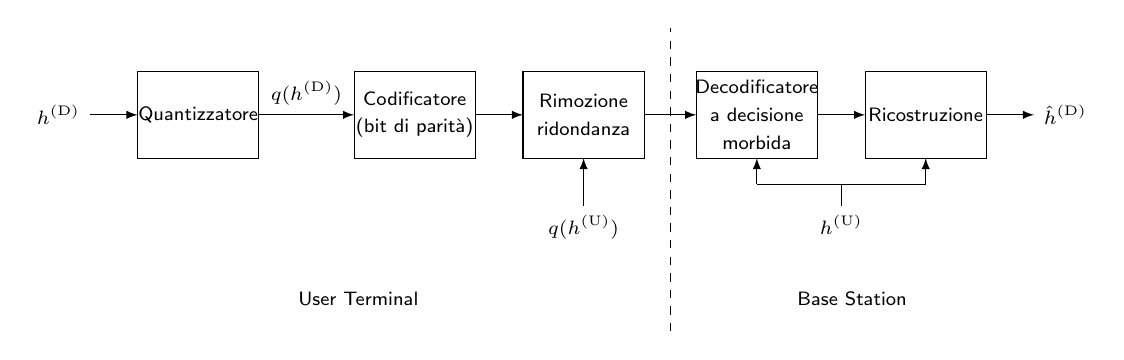
\begin{tikzpicture}[scale=0.55,>=latex]
    \tikzstyle{every node}=[font=\fontsize{6.8}{10}\sffamily]

    % Coding at UT
    \draw[->] (1.1,5) node[left]{\(\bm{h}^\mathrm{(D)}\)} -- (2.2,5);

    \draw (2.2,4) rectangle (5,6)
    node[midway,align=center]{Quantizzatore};

    \draw[->] (5,5) -- (7.2,5)
    node[above,midway]{\(q(\bm{h}^\mathrm{(D)})\)};

    \draw (7.2,4) rectangle (10,6)
    node[midway,align=center]{Codificatore \\ (bit di parità)};

    \draw[->] (10,5) -- (11.1,5);

    \draw (11.1,4) rectangle (13.9,6)
    node[midway,align=center]{Rimozione \\ ridondanza};

    \draw[->] (12.5,2.9) node[below]{\(q(\bm{h}^\mathrm{(U)})\)} -- (12.5,4);

    % Send in Feedback
    \draw[->] (13.9,5) -- (15.1,5);
    \draw[-, dashed] (14.5,0) -- (14.5,7);
    \draw (7.3,0.75) node {User Terminal};
    \draw (18.7,0.75) node {Base Station};

    % Decoding at BS
    \draw (15.1,4) rectangle (17.9,6)
    node[midway,align=center]{Decodificatore \\ a decisione \\ morbida};

    \draw[->] (16.5,3.4) -- (16.5,4);

    \draw[->] (17.9,5) -- (19,5);

    \draw (19,4) rectangle (21.8,6)
    node[midway,align=center]{Ricostruzione};

    \draw[->] (20.4,3.4) -- (20.4,4);

    \draw[-] (16.5,3.4) -- (20.4,3.4);
    \draw[-] (18.45,2.9) node[below]{\(\bm{h}^\mathrm{(U)}\)} -- (18.45,3.4);

    \draw[->] (21.8,5) -- (22.9,5)
    node[right]{\(\hat{\bm{h}}^\mathrm{(D)}\)};
\end{tikzpicture}

    \caption{
        Schema della codifica di sorgente con distorsione per la trasmissione
        del canale di DL in feedback.
    }
    \label{fig:procedure-schema}
\end{figure}
\newline
Il decodificatore a decisione morbida infatti può utilizzare un'informazione a
priori sulla distribuzione delle parole di codice. Questa distribuzione è
ottenuta dalla conoscenza del canale di UL e dalla correlazione di quest'ultimo
con il canale di DL.

